\chapter{3D geometry} \label{ch:3d-geometry}
We will in this chapter describe how we can relate different objects in 3D by defining local coordinate frames and transformations between them.
This will let us express the orientation and pose of objects relative to each other, which we can use to transform points between coordinate frames.
We will also introduce notation that makes the direction of these transformations explicit and easy to deduce.


\section{Points and coordinate frames} \label{sec:points-coordinate-frames}
\begin{figure}[htb]
    \centering
    \tdplotsetmaincoords{60}{110}
\begin{tikzpicture}[scale=2, tdplot_main_coords]
  \coordinate (O) at (0,0,0);
  \coordinate (P) at (0,4,2);
  
  \draw[thick, color=red, ->] (O) -- (1,0,0);
  \draw[thick, color=red, ->] (O) -- (0,1,0);
  \draw[thick, color=red, ->] (O) -- (0,0,1);
  \node[anchor=north, color=red] (Fa) at (0,0.1,-0.1) {$\cF_a \;$};
  
  \path (P) node[circle, fill, inner sep=1]{};
  \draw[-stealth, color=red] (O) -- (P)  node [midway, above] {$\vecx^a$};
  \node[anchor=west] at (P) {$X$};
\end{tikzpicture}

    \caption{A point $X$ represented by a vector $\vecx^a$ in the coordinate frame $\cF_a$.}
    \label{fig:coordinate_frame}
\end{figure}
A point in space may be described by a \emph{coordinate vector}, as shown in Figure \ref{fig:coordinate_frame}.
In this example, the point $X$ is described by the vector $\vecx^a \in \bbR^3$, which represents the displacement of the point in Euclidean space with respect to the \emph{coordinate frame} $\cF_a$.
A \emph{Cartesian coordinate frame} defines a set of orthogonal axes which intersect at a point called the origin.

An alternative to Cartesian coordinates in Euclidean space is to describe points using \emph{homogeneous coordinates} in projective space.
A homogeneous coordinate vector in projective space is given by $\tilde{\vecx} = [\tilde{x}, \tilde{y}, \tilde{z}, \tilde{w}]\trans \in \bbP^3$, where $\tilde{\vecx} = \lambda \tilde{\vecx}$ for all non-zero scalars $\lambda$.

Given a Cartesian coordinate vector $\vecx = [x, y, z]\trans \in \bbR^3$, we can represent the same point as the homogeneous coordinate vector $\tilde{\vecx} = \lambda[x, y, z, 1]\trans$.
This means that we can construct a homogeneous vector from a Cartesian vector with the mapping
\begin{equation} \label{eq:cart-to-homo}
  \vecx = 
  \begin{bmatrix}
  x\\
  y\\
  z
  \end{bmatrix}
  \in \bbR^3
  \quad \mapsto \quad
  \tilde{\vecx} = \breve{\vecx} =
  \begin{bmatrix}
  x\\
  y\\
  z\\
  1
  \end{bmatrix}
  \in \bbP^3,
\end{equation}
where we use the notation $\breve{\vecx}$ for the \emph{normalised} homogeneous coordinate $\breve{\vecx} = \begin{bsmallmatrix}\vecx\\ 1\end{bsmallmatrix}$, according to \emph{Euclidean normalisation}.
We can map a homogeneous vector back into a Cartesian vector with
\begin{equation} \label{eq:homo-to-cart}
  \tilde{\vecx} =
  \begin{bmatrix}
  \tilde{x}\\
  \tilde{y}\\
  \tilde{z}\\
  \tilde{w}
  \end{bmatrix}
  \in \bbP^3
  \quad \mapsto \quad
  \vecx = 
  \begin{bmatrix}
  \tilde{x} / \tilde{w}\\
  \tilde{y} / \tilde{w}\\
  \tilde{z} / \tilde{w}
  \end{bmatrix}
  \in \bbR^3.
\end{equation}
Homogeneous vectors with $\tilde{w} = 0$ have no representation in $\bbR^3$, and correspond to the direction to points infinitely far away from the origin.
As we will see later, homogeneous coordinates are a convenient representation when describing transformations and camera projections of points and directions.
See Hartley and Zisserman \cite{Hartley2004MultipleVision} for a detailed description of projective geometry for computer vision.

\begin{figure}[htb]
    \centering
    \tdplotsetmaincoords{60}{110}
\begin{tikzpicture}[scale=2, tdplot_main_coords]
  \coordinate (O) at (0,0,0);
  \coordinate (P) at (0,4,2);
  
  \draw[thick, color=red, ->] (O) -- (1,0,0);
  \draw[thick, color=red, ->] (O) -- (0,1,0);
  \draw[thick, color=red, ->] (O) -- (0,0,1);
  \node[anchor=north, color=red] (Fa) at (0,0.1,-0.1) {$\cF_a \;$};
  
  \path (P) node[circle, fill, inner sep=1]{};
  \node[anchor=west] at (P) {$X$};
  
  \draw[-stealth, color=red] (O) -- (P)  node [midway, above] {$\vecx^a$};
  
  \coordinate (W) at (3, 3, 1);
  \tdplotsetrotatedcoords{30}{0}{0};
  \tdplotsetrotatedcoordsorigin{(W)};
  
  \draw[thick, color=green!50!black, tdplot_rotated_coords,->] (0,0,0) -- (1,0,0);
  \draw[thick, color=green!50!black, tdplot_rotated_coords,->] (0,0,0) -- (0,1,0);
  \draw[thick, color=green!50!black, tdplot_rotated_coords,->] (0,0,0) -- (0,0,1);
  \node[anchor=north east, color=green!50!black, tdplot_rotated_coords] (Fb) at (0,0,0) {$\cF_b \;$};
  
  \draw[-stealth, tdplot_rotated_coords, color=green!50!black] (0,0,0) -- (P)  node [midway, above] {$\vecx^b$};
  
  \draw[-stealth, densely dotted] (Fa)  to [bend right=60]  node [midway, below] {$\matT_{ab}$} (Fb);
  
  
\end{tikzpicture}

    \caption{A point $X$ represented by a vector $\vecx^a$ in the coordinate frame $\cF_a$, and a corresponding vector $\vecx^b$ in the coordinate frame $\cF_b$.
    The pose $\matT_{ab}$ describes the position and orientation of $\cF_b$ relative to $\cF_a$.}
    \label{fig:more_frames}
\end{figure}
It is sometimes necessary to describe the same point relative to several coordinate frames.
We might for example want to relate a point given in a world frame to the local coordinate frame of a camera.
The relationship between the Cartesian coordinate frames in Figure~\ref{fig:more_frames} can be described by the \emph{position} and \emph{orientation} of $\cF_b$ relative to $\cF_a$.
This is also called the \emph{pose} of $\cF_b$ relative to $\cF_a$, and can be expressed as a transformation $\matT_{ab}$ that lets us map the point's coordinates $\vecx^b$ in $\cF_b$ to coordinates $\vecx^a$ in $\cF_a$.

We will in the following sections see how we can represent and apply such transformations between coordinate frames.


\section{Representing orientation} \label{sec:orientation}
\begin{figure}[htb]
    \centering
    \tdplotsetmaincoords{60}{110}
\begin{tikzpicture}[scale=2, tdplot_main_coords]
  \coordinate (O) at (0,0,0);
  
  \draw[thick, color=red,->] (O) -- (1,0,0) node[anchor=north east]{$\veca_1$};
  \draw[thick, color=red,->] (O) -- (0,1,0) node[anchor=south west]{$\veca_2$};
  \draw[thick, color=red,->] (O) -- (0,0,1) node[anchor=south east]{$\veca_3$};
  \node[anchor=east, color=red] (Fa) at (O) {$\cF_a \;$};
  
  \tdplotsetrotatedcoords{45}{20}{20};
  
  \draw[thick, color=green!50!black, tdplot_rotated_coords,->] (0,0,0) -- (1,0,0) node[anchor=north]{$\vecb_1$};
  \draw[thick, color=green!50!black, tdplot_rotated_coords,->] (0,0,0) -- (0,1,0) node[anchor=west]{$\vecb_2$};
  \draw[thick, color=green!50!black, tdplot_rotated_coords,->] (0,0,0) -- (0,0,1) node[anchor=south west]{$\vecb_3$};
  \node[anchor=north, color=green!50!black] (Fb) at (0.2,0.2,0) {$\cF_b \;$};
  
  \draw[-stealth, densely dotted] (Fa)  to [bend right=60]  node [near start, left] {$\matR_{ab}$} (Fb);
  
\end{tikzpicture}

    \caption{Two coordinate frames $\cF_a$ and $\cF_b$ with the same origin. The orientation of $\cF_b$ relative to $\cF_a$ is described by the rotation matrix $\matR_{ab}.$}
    \label{fig:rotated_frames}
\end{figure}

We can describe the orientation of coordinate frame $\cF_b$ relative to $\cF_a$ by how we should rotate $\cF_a$ in order to align with $\cF_b$.
This rotation has 3 degrees of freedom (DOF), and can be represented by the orthogonal rotation matrix
\begin{equation}
  \matR_{ab} = 
  \begin{bmatrix}
  r_{11} & r_{12} & r_{13}\\
  r_{21} & r_{22} & r_{23}\\
  r_{31} & r_{32} & r_{33}
  \end{bmatrix}
  \in \SO(3).
\end{equation}
Rotation matrices belong to the $\SO(3)$ Lie group (special orthogonal group of dimension 3), which we will cover in more detail in Section \ref{sec:SO3_group}.

Let the coordinate frame $\cF_a$ be defined by the orthonormal basis vectors $\{\veca_1, \veca_2, \veca_3\}$, and the frame $\cF_b$ be defined by the orthonormal basis vectors $\{\vecb_1, \vecb_2, \vecb_3\}$, as illustrated in Figure \ref{fig:rotated_frames}.
The columns of the rotation matrix representing the orientation of $\cF_b$ relative to $\cF_a$ correspond to the basis vectors of $\cF_b$ expressed in frame $\cF_a$
\begin{equation} \label{eq:rot_basis}
  \matR_{ab} = 
  \begin{bmatrix}
    \vecb^a_1 & \vecb^a_2 & \vecb^a_3
  \end{bmatrix}.
\end{equation}
When the coordinate frames have the same origin, this lets us use the orientation of $\cF_b$ relative to $\cF_a$ to transform points $\vecx^b$ given in frame $\cF_b$ to points $\vecx^a$ given in frame $\cF_a$ by
\begin{equation}
  \vecx^a = \matR_{ab} \vecx^b.
\end{equation}

\begin{figure}[htb]
    \centering
    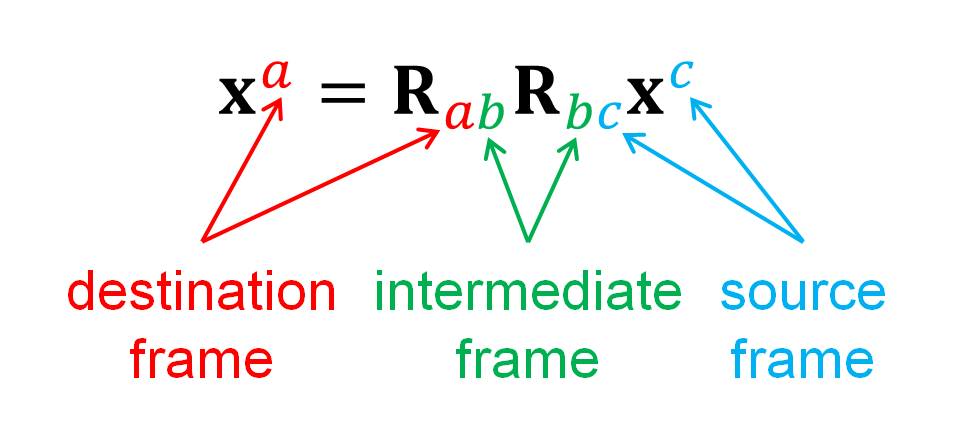
\includegraphics[width=0.5\columnwidth]{figures/coordinate_frame_notation.png}
    \caption{The coordinate frame notation helps us combine transformations in the correct order.}
    \label{fig:coordinate-frame-notation}
\end{figure}

We can also compose relative orientations with matrix multiplication
\begin{equation}
  \matR_{ac} = \matR_{ab} \matR_{bc}.
\end{equation}
The inverse orientation is given by the inverse rotation matrix, and since rotation matrices are orthogonal, we have
\begin{equation}
  \matR_{ba} = \matR_{ab}^{-1} = \matR_{ab}\trans.
\end{equation}
Notice in Figure \ref{fig:coordinate-frame-notation} how the subscript and superscript notation for coordinate frames aligns, and helps us combine transformations in the correct order.

\begin{example}[frametitle=Transforming detections between sensors]
{
  \centering
  \tdplotsetmaincoords{10}{45}
\begin{tikzpicture}[scale=2, tdplot_main_coords]
  \coordinate (O) at (0,0,0);
  \coordinate (P) at (1.75,2.25,0);
  
  \draw[thick, color=green!50!black,->] (O) -- (1,0,0);
  \draw[thick, color=green!50!black,->] (O) -- (0,1,0);
  \draw[thick, color=green!50!black,->] (O) -- (0,0,1);
  \node[anchor=east, color=green!50!black, tdplot_screen_coords] (Fb) at (-0.3, 0, 0) {$\cF_b \;$};
  
  \tdplotsetrotatedcoords{-30}{-10}{0};
  \draw[thick, color=blue, tdplot_rotated_coords,->] (0,0,0) -- (1,0,0);
  \draw[thick, color=blue, tdplot_rotated_coords,->] (0,0,0) -- (0,1,0);
  \draw[thick, color=blue, tdplot_rotated_coords,->] (0,0,0) -- (0,0,1);
  \node[anchor=east, color=blue, tdplot_screen_coords] (Fc) at (-0.3, -0.75) {$\cF_c \;$};
  \draw[-stealth, tdplot_rotated_coords, color=blue] (0,0,0) -- (P)  node [near end, above] {$\vecx^c$};
  \path (P) node[circle, fill, inner sep=1]{};
  \node[anchor=west] at (P) {$X$};
  
  \tdplotsetrotatedcoords{30}{10}{10};
  \draw[thick, color=red, tdplot_rotated_coords,->] (0,0,0) -- (1,0,0);
  \draw[thick, color=red, tdplot_rotated_coords,->] (0,0,0) -- (0,1,0);
  \draw[thick, color=red, tdplot_rotated_coords,->] (0,0,0) -- (0,0,1);
  \node[anchor=east, color=red, tdplot_screen_coords] (Fa) at (-0.3, 0.75) {$\cF_a \;$};
  
  \draw[-stealth, densely dotted] (Fb)  to [bend left=60]  node [midway, left] {$\matR_{ba}$} (Fa);
  \draw[-stealth, densely dotted] (Fb)  to [bend right=60]  node [midway, left] {$\matR_{bc}$} (Fc);
  
  
\end{tikzpicture}

  \captionsetup{type=figure}
  \captionof{figure}{Three differently oriented sensors.}
  \label{fig:orientation_example}
  \par
}

Assume that we have three coordinate frames $\cF_a$, $\cF_b$ and $\cF_c$ at the same origin, as shown in Figure~\ref{fig:orientation_example}.
These correspond to three co-located, but differently oriented sensors.
The sensor system has been calibrated with regards to sensor $b$, so we are given $\matR_{ba}$ and $\matR_{bc}$.
When the sensor $c$ detects a point $\vecx^c$ represented in frame $\cF_c$, what is the corresponding position in the coordinate frame of sensor $a$?

We can represent the relative orientation between $\cF_c$ and $\cF_a$ using the calibrated orientations by
\begin{equation}
  \matR_{ac} = \matR_{ab} \matR_{bc} = \matR_{ba}\trans \matR_{bc}.
\end{equation}
This lets us compute the point represented in $\cF_a$ as
\begin{equation}
  \vecx^a = \matR_{ac} \vecx^c = \matR_{ba}\trans \matR_{bc} \vecx^c.
\end{equation}
\end{example}

Since $\matR_{ba} = \matR_{ab}\trans$, we see from \eqref{eq:rot_basis} that the rows of $\matR_{ba}$ are given by the basis vectors of $\cF_a$ expressed in frame $\cF_b$
\begin{equation} \label{eq:rot_basis_rows}
  \matR_{ab} = 
  \begin{bmatrix}
    {\veca^b_1}\trans\\
    {\veca^b_2}\trans\\
    {\veca^b_3}\trans
  \end{bmatrix}.
\end{equation}
This is sometimes useful when assessing how coordinate systems relate to each other.

\begin{example}[frametitle=Rotation matrix from basis vector perturbations]
{
  \centering
  \tdplotsetmaincoords{-120}{70}
\begin{tikzpicture}[scale=2, tdplot_main_coords]
  \coordinate (O) at (0,0,0);
  
  \draw[thick, color=red,->] (O) -- (1,0,0) node[anchor=south east]{$\veca_1$};
  \draw[thick, color=red,->] (O) -- (0,1,0) node[anchor=south west]{$\veca_2$};
  \draw[thick, color=red,->] (O) -- (0,0,1) node[anchor=north west]{$\veca_3$};
  \node[anchor=east, color=red] (Fa) at (0.2, -0.1, 0) {$\cF_a \;$};
  
  \tdplotsetrotatedcoords{0}{90}{90};
  
  \draw[thick, dashed, color=green!50!black, tdplot_rotated_coords,->] (0,0,0) -- (1,0,0) node[anchor=north]{$\vecb_1$};
  \draw[thick, dashed, color=green!50!black, tdplot_rotated_coords,->] (0,0,0) -- (0,1,0) node[anchor=east]{$\vecb_2$};
  \draw[thick, dashed, color=green!50!black, tdplot_rotated_coords,->] (0,0,0) -- (0,0,1) node[anchor=west]{$\vecb_3$};
  \node[anchor=north, color=green!50!black] (Fb) at (0,0.2,0.1) {$\cF_b \;$};
  
  \draw[-stealth, densely dotted] (Fa)  to [bend right=60]  node [midway, left] {$\matR_{ab}$} (Fb);
  
\end{tikzpicture}

  \captionsetup{type=figure}
  \captionof{figure}{Two coordinate frames with their corresponding basis vectors.}
  \label{fig:perturbed_basis_example}
  \par
}

As shown in Figure \ref{fig:perturbed_basis_example}, we have a coordinate frame $\cF_a$, where the $x$-axis points forwards, the $y$-axis points right and the $z$-axis points down.
We also have a coordinate frame $\cF_b$ where the $z$-axis points forwards and the $x$-axis points right.
What is the orientation $\matR_{ab}$ of $\cF_b$ relative to $\cF_a$?

From \eqref{eq:rot_basis} we know that the columns of $\matR_{ab}$ correspond to the basis vectors of $\cF_b$ relative to $\cF_a$.
Since $\vecb^a_1 = \veca_2$, $\vecb^a_2 = \veca_3$ and $\vecb^a_3 = \veca_1$, we get
\begin{equation} \label{eq:rot_basis_example}
  \matR_{ab} = 
  \begin{bmatrix}
    \veca_2 & \veca_3 & \veca_1
  \end{bmatrix}
  =
  \begin{bmatrix}
    0 & 0 & 1\\
    1 & 0 & 0\\
    0 & 1 & 0
  \end{bmatrix}.
\end{equation}

With \eqref{eq:rot_basis_rows}, we can now also confirm that the rows of \eqref{eq:rot_basis_example} correspond to the basis vectors of $\cF_a$ relative to $\cF_b$.
\end{example}

Rotations about the basis vectors are called \emph{principal rotations}.
The rotation matrices for a rotation $\theta$ about the $x$-, $y$- and $z$-axes are given by
\begin{align}
  \matR_x(\theta) &= 
  \begin{bmatrix}
    1 & 0 & 1\\
    0 & \cos \theta & -\sin \theta\\
    0 & \sin \theta & \cos \theta
  \end{bmatrix}\\[1em]
  %
  \matR_y(\theta) &= 
  \begin{bmatrix}
    \cos \theta & 0 & \sin \theta\\
    0 & 1 & 0\\
    -\sin \theta & 0 & \cos \theta
  \end{bmatrix}\\[1em]
  %
  \matR_z(\theta) &= 
  \begin{bmatrix}
    \cos \theta & -\sin \theta & 0\\
    \sin \theta & \cos \theta & 0\\
    0 & 0 & 1
  \end{bmatrix}.
\end{align}
Any orientation can be represented by a sequence of three principal rotations, where no two successive rotations are about the same axis.
This lets us specify an orientation as a set of three angles $(\theta_1, \theta_2, \theta_3)$ and a corresponding sequence of principal rotations, which is often referred to as the Euler angle representation.

\begin{example}[frametitle={Orientation represented as roll, pitch and yaw}]
{
  \centering
  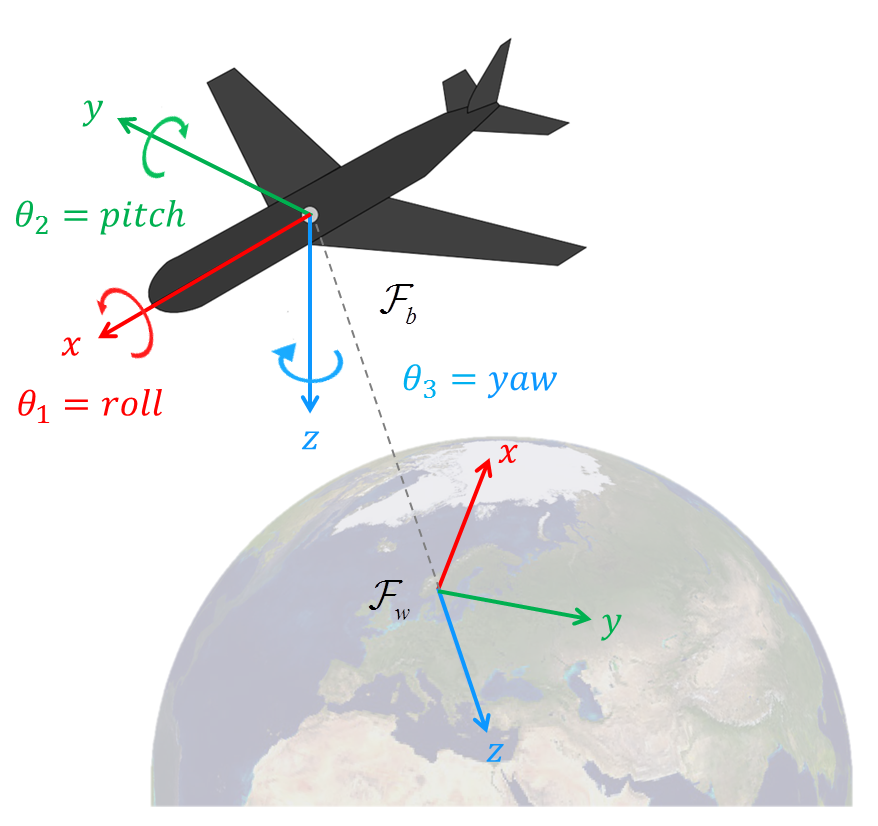
\includegraphics[width=0.5\columnwidth]{figures/roll-pitch-yaw_NED.png}
  \captionsetup{type=figure}
  \captionof{figure}{The orientation of the body frame $\cF_b$ (front, right, down) relative to the world frame $\cF_w$ (north, east, down) is represented with roll-, pitch- and yaw-angles about the body axes.}
  \label{fig:roll-pitch-yaw_example}
  \par
}

We have an aircraft with body coordinate frame $\cF_b$, where the $x$-axis points forward, the $y$-axis points right and the $z$-axis points down.
The world coordinate frame $\cF_w$ is given as a NED frame, where the $x$-axis points north, the $y$-axis points east and the $z$-axis points down.
The roll-, pitch- and yaw-angles around the principal axes of $\cF_b$ are given as $(\theta_1, \theta_2, \theta_3)$, as shown in Figure \ref{fig:roll-pitch-yaw_example}.

We can compute the rotation matrix corresponding to the orientation of $\cF_b$ relative to $\cF_w$ with the roll-pitch-yaw sequence of principal rotations
\begin{equation}
  \matR_{wb} = \matR_z(\theta_3) \matR_y(\theta_2) \matR_x(\theta_1).
\end{equation}
\end{example}

It is also possible to describe any orientation as a rotation about a given axis.
This is called the \emph{angle-axis} representation, and can be expressed as
\begin{equation}
  \vectheta = \theta \vecu,
\end{equation}
where $\theta$ is the angle of rotation and $\vecu$ is the unit-length axis of rotation.
The corresponding rotation matrix is given by Rodrigues' rotation formula
\begin{equation} \label{eq:rot-from-axis-angle}
  \matR(\vectheta) = \matI + \sin \theta [\vecu]_\times + (1 - \cos \theta) [\vecu]^2_\times, 
\end{equation}
where $[\vecu]_\times$ is the skew-symmetric matrix\footnotemark
\begin{equation}
  [\vecu]_\times =
  \begin{bmatrix}
    u_1\\
    u_2\\
    u_3
  \end{bmatrix}_\times \triangleq
  \begin{bmatrix}
    0 & -u_3 & u_2\\
    u_3 & 0 & -u_1\\
    -u_2 & u_1 & 0
  \end{bmatrix}.
\end{equation}
When the angle $\theta$ is small, the corresponding rotation matrix can be approximated with the matrix
\begin{equation} \label{eq:infinitesimal-rotaton}
  \matR(\vectheta) \approx \matI + [\vectheta]_\times.
\end{equation}
This is sometimes called an \emph{infinitesimal rotation}.
\footnotetext{The cross product between two vectors can also be represented as a matrix multiplication using this skew-symmetric matrix: $\veca \times \vecb = [\veca]_\times \vecb$. This explains the common $[\cdot]_\times$ notation.}

Another similar and very popular representation for rotation is the \emph{unit quaternion}, which is covered in detail in e.g. \cite{barfoot2017state}.

The orthogonal rotation matrix has 9 elements that parameterise the 3 DOF rotation.
The Euler angle and angle-axis representations are both minimal representations, in that they both can be represented by 3 parameters, but they suffer from singularities.
In fact, there is no perfect representation that is minimal and also free of singularities.
This is because 3D rotations lie on a 3D manifold embedded in a higher dimensional space.
We will in Chapters~\ref{sec:Lie-theory},~\ref{ch:jacobians} and \ref{ch:uncertainty} see how we can describe perturbations, derivatives and probability distributions on this manifold.

\section{Representing pose}
\begin{figure}[htb]
    \centering
    \tdplotsetmaincoords{60}{110}
\begin{tikzpicture}[scale=2, tdplot_main_coords]
  \coordinate (O) at (0,0,0);
  
  \draw[thick, color=red, ->] (O) -- (1,0,0);
  \draw[thick, color=red, ->] (O) -- (0,1,0);
  \draw[thick, color=red, ->] (O) -- (0,0,1);
  \node[anchor=north, color=red] (Fa) at (0,0.1,-0.1) {$\cF_a \;$};
  
  \coordinate (W) at (3, 3, 1);
  \tdplotsetrotatedcoords{30}{0}{0};
  \tdplotsetrotatedcoordsorigin{(W)};
  
  \draw[thick, color=green!50!black, tdplot_rotated_coords,->] (0,0,0) -- (1,0,0);
  \draw[thick, color=green!50!black, tdplot_rotated_coords,->] (0,0,0) -- (0,1,0);
  \draw[thick, color=green!50!black, tdplot_rotated_coords,->] (0,0,0) -- (0,0,1);
  \node[anchor=north east, color=green!50!black, tdplot_rotated_coords] (Fb) at (0,0,0) {$\cF_b \;$};
  
  \draw[-stealth, densely dotted] (Fa)  to [bend right=60]  node [midway, below] {$\matR_{ab}$} (Fb);
  \draw[-stealth, color=red] (O) -- (W)  node [near end, above] {$\vect^a_{ab}$};
  
\end{tikzpicture}

    \caption{Two coordinate frames $\cF_a$ and $\cF_b$ with different position and orientation. The pose of $\cF_b$ relative to $\cF_a$ is described by the orientation $\matR_{ab}$ and the translation $\vect^a_{ab}$ between the frame origins.}
    \label{fig:pose-illustration}
\end{figure}

When coordinate frames do not share a common origin, we also need to take the relative position between frames into account.
The \emph{pose} of $\cF_b$ relative to $\cF_a$ describes how $\cF_a$ should be rotated \emph{and} translated in order to coincide with $\cF_b$.
This can be represented with the homogeneous transformation matrix
\begin{equation}
  \matT_{ab} = 
  \begin{bmatrix}
  \matR_{ab} & \vect^a_{ab}\\[0.3em]
  \matr{0}\trans & 1
  \end{bmatrix}
  \in \SE(3),
\end{equation}
where $\matR_{ab} \in \SO(3)$ represents the orientation of $\cF_b$ relative to $\cF_a$, and $\vect^a_{ab} \in \bbR^3$ is a translation vector given in the coordinate frame of $\cF_a$.
This vector represents the position of $\cF_b$ relative to $\cF_a$, as shown in Figure \ref{fig:pose-illustration}.
The $4 \times 4$ pose matrices are known as \emph{3D Euclidean} or \emph{3D rigid body} transformations, and belong to the $\SE(3)$ Lie group (special Euclidean group of dimension 3), which we will cover in more detail in Section \ref{sec:SE3_group}.

The fact that $\matT$ is a homogeneous transformation matrix means that we can express the Euclidean transformation linearly using homogeneous vectors.
Given a point $\vecx^b$ represented in $\cF_b$ and the pose $\matT_{ab}$ of $\cF_b$ relative to $\cF_a$, we can convert to the homogeneous representation $\tilde{\vecx}^b$ using \eqref{eq:cart-to-homo}, and transform the point to coordinates given in frame $\cF_a$ by
\begin{equation} \label{eq:homo-pose-transf}
  \tilde{\vecx}^a = \matT_{ab} \tilde{\vecx}^b.
\end{equation}
We get the Cartesian coordinate $\vecx^a$ by normalising $\tilde{\vecx}^a$ according to \eqref{eq:homo-to-cart}.

The transformation in \eqref{eq:homo-pose-transf} corresponds to rotating $\vecx^b$ into frame $\cF_a$, and translating according to the position of $\cF_b$ relative to $\cF_a$.
We can therefore express the transformation equivalently on Cartesian form as
\begin{equation}
  \vecx^a = \matR_{ab} \vecx^b + \vect^a_{ab}.
\end{equation}
%Although this form is less concise, we avoid the use of homogeneous coordinates, and can operate on the orientation $\matR$ and translation $\vect$ directly.
We will call this transformation the \emph{action} of the pose $\matT$ on the vector $\vecx$, and denote it as $\matT \cdot \vecx$, where
\begin{equation}
  \vecx^a = \matT_{ab} \cdot \vecx^b = \matR_{ab} \vecx^b + \vect^a_{ab}.
\end{equation}

As for rotations, we can compose relative poses with matrix multiplication.
This can also be expressed directly as operations on $\matR$ and $\vect$ by
\begin{equation}
  \matT_{ac} = \matT_{ab} \matT_{bc} =
  \begin{bmatrix}
    \matR_{ab} \matR_{bc} & \matR_{ab} \vect^b_{bc} + \vect^a_{ab}\\[0.3em]
    \matr{0}\trans & 1
  \end{bmatrix}
\end{equation}
The inverse pose is given by
\begin{equation}
  \matT_{ba} = \matT_{ab}^{-1} = 
  \begin{bmatrix}
    \matR_{ab}\trans  & -\matR_{ab}\trans \vect^a_{ab}\\[0.3em]
    \matr{0}\trans & 1
  \end{bmatrix}.
\end{equation}

Since all pose operations can be expressed as operations on the orientation and position directly, it is common to implement poses in practice as a pair $(\matR, \vect)$, rather than the full matrix $\matT$.
This avoids the use of homogeneous coordinates, and allows alternative representations for orientation, such as quaternions.
This dual representation lets us exploit the mathematical properties of $\matT$, while simultaneously reaping the benefits of the chosen implementation for orientation and pose operations.

\begin{example}[frametitle=Seeing a point in the world with a camera]
{
  \centering
  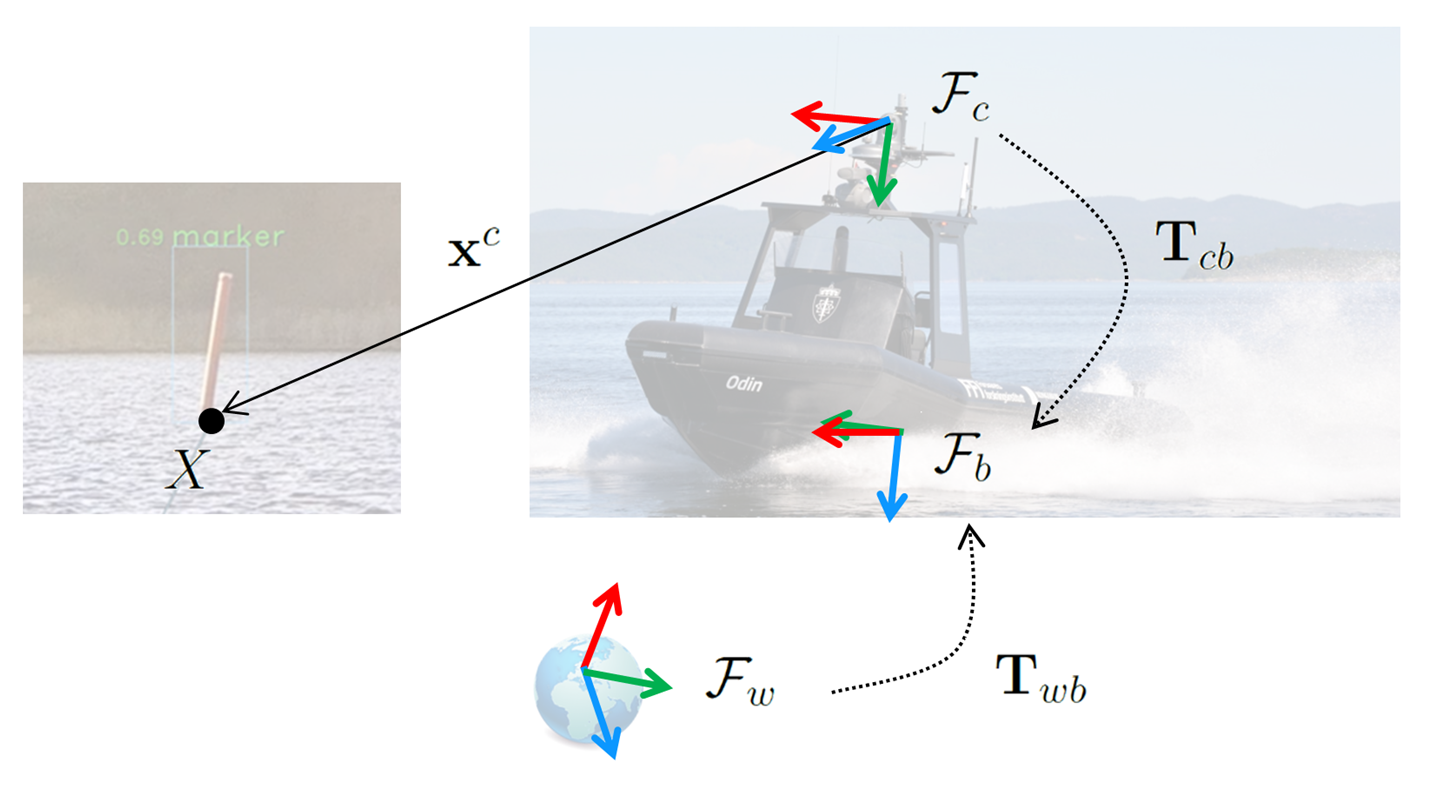
\includegraphics[width=0.75\columnwidth]{figures/odin_pose_example.png}
  \captionsetup{type=figure}
  \captionof{figure}{A camera observes a sea marker in the camera frame $\cF_c$. A navigation system estimates the pose of the boat relative to the world frame $\matT_{wb}$, and the pose of the boat relative to the camera $\matT_{cb}$ is known.}
  \label{fig:odin_pose_example}
  \par
}

An autonomous boat observes a sea marker in its camera frame $\cF_c$.
As illustrated in Figure~\ref{fig:odin_pose_example}, we are given the pose of the boat relative to the world frame $\matT_{wb}$, as well as the pose of the boat relative to the camera frame $\matT_{cb}$.
Where is the sea marker relative to the world frame $\cF_w$?

We can compute the pose of the camera relative to the world by
\begin{subequations}
\begin{align}
  \matT_{wc} &= \matT_{wb} \matT_{bc}\\
  &= \matT_{wb} \matT_{cb}^{-1}\\
  &=
  \begin{bmatrix}
    \matR_{wb} \matR_{cb}\trans  & -\matR_{wb} \matR_{cb}\trans \vect^c_{cb} + \vect^w_{wb}\\[0.3em]
    \matr{0}\trans & 1
  \end{bmatrix}.
\end{align}
\end{subequations}
The coordinate of the sea marker in the world frame is then
\begin{equation}
  \tilde{\vecx}^w = \matT_{wc} \tilde{\vecx}^c = \matT_{wb} \matT_{cb}^{-1} \tilde{\vecx}^c,
\end{equation}
or equivalently
\begin{subequations}
\begin{align}
  \vecx^w &= \matT_{wc} \cdot \vecx^c\\
  &= \matR_{wc} \vecx^c + \vect^w_{wc}\\
  &= \matR_{wb} \matR_{cb}\trans \vecx^c - \matR_{wb} \matR_{cb}\trans \vect^c_{cb} + \vect^w_{wb}.
\end{align}
\end{subequations}
\end{example}
